\subsection{BPMS: Camunda}
Il meccanismo di interazione tra il sistema (in altre parole, l'azienda
ACME) e l'utente \`e stata gestita tramite la piattaforma Camunda.
Per implementare tale meccanismo si \`e partiti da una versione
semplificata dal BPMN descritto in precedenza, in modo tale da poter
correttamente inserire gli elementi necessari a Camunda e nascondere le
parti dello schema implementate dalla SOA di servizi Jolie, dunque non
gestita da Camunda.

Come prima cosa il cliente deve avviare il processo, inviando un ordine
tramite la pagina HTML che simula la grafica e le meccaniche del sito
internet della ACME.
Il cliente deve autenticarsi all'interno del sito e comporre un ordine.
Una volta controllato che un ordine sia coerente, cio\`e che tutti i
prodotti richiesti esistano e che tutte le customizzazioni richieste
siano compatibili, allora il sistema invia una email al cliente che
l'ordine \`e stato preso in carico.
Si \`e deciso di utilizzare come identificativo dell'ordine, in tutti
questi passaggi, l'ID del processo Camunda, poich\'e garantisce
univocit\`a certa.
Le comunicazioni con il cliente sono state tutte implementate tramite
l'invio di email: l'indirizzo viene infatti ricavato dai dati di login
utilizzati dal cliente stesso all'interno del sito.

Informato il cliente dell'accettazione dell'ordine, si delega il lavoro
alla SOA di servizi Jolie descritta nel dettaglio in seguito.
Per comunicare con i servizi Jolie addetti alla gestione del magazzino
\`e stato necessario utilizzare il protocollo {\tt soap}, implementando
classi apposite ({\tt package: it.unibo.isos.soap}). Tali classi
permettono di gestire le comunicazioni tra ufficio e magazzino
correttamente.

Dalla SOA di servizi Jolie arrivano spesso dei messaggi utili agli
utilizzatori del sistema: per esempio, quando viene composto il
preventivo della vendita, se esso supera una certa cifra, viene
richiesto ad un operatore se si desidera imporre uno sconto, in
percentuale.
Tale meccanismo viene gestito da Camunda con il sistema degli
\textit{User Task}.
\begin{figure}
  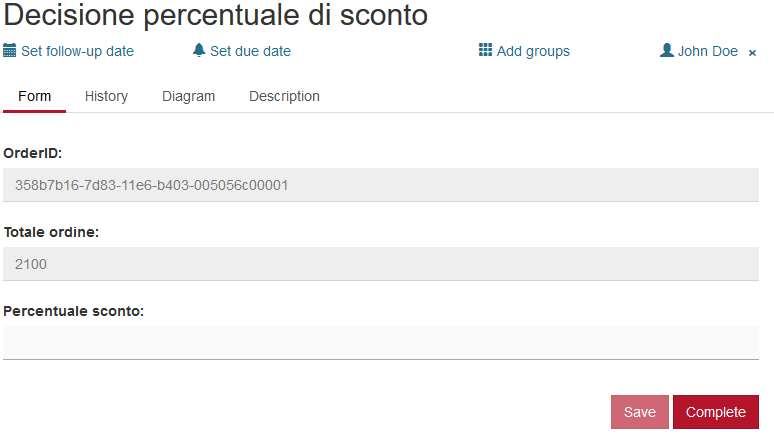
\includegraphics[scale=0.6]{immagini/camunda_percentuale_sconto.PNG}
  \captionsetup{labelformat=empty}
  \caption{Decisione della percentuale di sconto.}
\end{figure}

Concluso questo passaggio, il cliente riceve una email contenente il
preventivo e due link: uno per accettare il prezzo proposto dalla ACME,
un altro per rifiutare lo stesso.
Entrambi i link puntano ad una {\tt servlet} che si occupa di inviare un
messaggio al processo che gestisce l'ordine del cliente.

Effettuati i vari passaggi legati all'accettazione del preventivo, viene
gestito, tramite \textit{subprocess}, il corretto pagamento della
caparra. Per simulare un sistema realistico senza dover attendere intere
ore prima di verificare un pagamento, si \`e deciso di utilizzare timer
nell'ordine dei minuti.
Dopo \textit{n} minuti, infatti, tali subprocess controllano se il
cliente ha effettuato il pagamento.
Intorno a questo timer di verifica ne \`e stato implementato uno pi\`u
lungo, che controlla che il pagamento avvenga entro il tempo utile per
validare l'ordine.

Come ultimo passaggio, la SOA di servizi Jolie si occupa di amministrare
tutto ci\`o che \`e connesso all'assemblaggio, alla spedizione e alla
gestione delle quantit\`a di prodotti nei magazzini, interagendo con le
varie capability esterne descritte successivamente.

Infine avviene il controllo del pagamento del saldo da parte del
cliente: se tutto \`e andato a buon fine, viene inviata una email al
cliente per comunicare l'esito positivo e si archivia l'ordine. Nel caso
ci siano invece stati dei problemi legati al pagamento del saldo, viene
notificato l'ufficio legale.

\subsubsection{Servizio e-mail}
Componente interessante di questo sistema \`e il servizio per l'invio
delle email, fondamentali nell'interazione con il cliente ed ottima
approssimazione delle comunicazioni cliente-azienda che avvengono nel
mondo reale.
Il servizio utilizzato, gratuito per un basso numero di email, \`e
\textit{mailgun} ({\tt www.mailgun.com}): per utilizzarlo vengono
fornite delle API, alle quali il sistema si interfaccia tramite la
classe {\tt SendMail}.
Nelle immagini si possono trovare alcuni esempi di email inviate dal
sistema.
\newpage
\begin{figure}
  
\includegraphics[scale=0.7]{immagini/email_annullamento_ordine.PNG}
  \captionsetup{labelformat=empty}
  \caption{Email di annullamento di un ordine.}
\end{figure}
\begin{figure}
  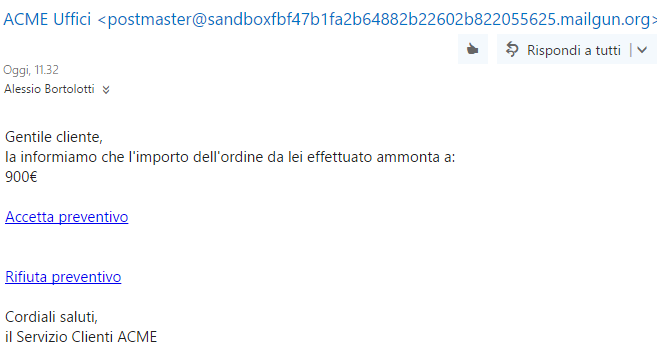
\includegraphics[scale=0.7]{immagini/email_preventivo.PNG}
  \captionsetup{labelformat=empty}
  \caption{Email di preventivo di un ordine.}
\end{figure}
\begin{figure}
  
\includegraphics[scale=0.7]{immagini/email_incompatibilita.PNG}
  \captionsetup{labelformat=empty}
  \caption{Email di un ordine con customizzazioni non compatibili.}
\end{figure}
\newpage
\subsubsection{User task}
Grazie all'implementazione di diversi user task \`e possibile per i
membri dell'ufficio avere una panoramica del sistema abbastanza
completa. Inn particolare sono stati implementati user task per:
\begin{itemize}
  \item ricezione di un nuovo ordine;
  \item annullamento di un ordine;
  \item accettazione/rifiuto di un ordine da parte di un cliente;
  \item spedizione di un ordine;
  \item archiviazione di un ordine;
  \item segnalazione di problemi connessi al pagamento di un ordine.
\end{itemize}
